% Provenance (never printed): see sources/outline_sources.md (Year 3: elastic waves
% recalled from the physics books; rays in a spherical Earth; travel-time tables;
% surface waves and dispersion; normal modes, told; linear inverse problems and
% seismic tomography). Brief: sources/book5/BRIEFS.md, ch. 1. Curves from
% figdata/bachelor-3/ray_tracing.py, love_dispersion.py, tomo_checkerboard.py;
% exercise and problem values in the Book 5 scratch calculator calc/ch01.py.
\chapter{Seismology and Earth Imaging}\label{ch:b3:seismology-imaging}

On 22 May 1960, at 19:11 universal time, the largest earthquake recorded since
1900 broke the subduction zone off southern Chile, with a magnitude of 9.5.
% ledger: usgs5:chile1960
Its P waves reached stations on the far side of the planet some twenty minutes
later; its surface waves went round the globe several times; and for days
afterwards the slowest instruments recorded the whole Earth vibrating with
periods close to an hour, like a struck bell. Each of these signals carries
information about the rocks it crossed. From the arrival times of millions of
such waves, read at thousands of stations, seismologists have built not only
the layered model of the Earth recalled below but three-dimensional images of
the mantle, in which sinking slabs and rising plumes appear as regions where
the waves travel slightly faster or slower than average. This chapter shows how:
how rays travel through a spherical Earth, how surface waves probe the crust
and mantle through their dispersion, how the free oscillations of the whole
planet are described, and how a few thousand travel times are turned into a
picture by solving a linear \omterm{def:b3:seismology-imaging:inverse}{inverse problem}.

\begin{recall}
In an isotropic elastic solid two kinds of body waves travel: P waves, at the
speed $\alpha = \sqrt{(K + \tfrac43\mu)/\rho}$, and S waves, at
$\beta = \sqrt{\mu/\rho}$, where $K$ and $\mu$ are the bulk and shear moduli
and $\rho$ the density; S waves do not cross a liquid (the physics books' Year 3
volume, in the chapter on continuum elasticity). A wave whose phase velocity
depends on its frequency is dispersive; its energy travels at the group
velocity $U = \mathrm d\omega/\mathrm dk$ (the physics books' Year 2 volume, on
waves). A bounded elastic body vibrates freely in a discrete set of normal
modes (same volume). The epicentral distance $\Delta$ of a station is the angle
at the Earth's centre between the epicentre and the station; the travel-time
curve gives the time of first arrival against $\Delta$, and the core casts a
shadow zone for direct P waves (Book 2, grade 11). The reference Earth model,
the seismic discontinuities and the head wave were met in the Year 1 volume,
in its chapter on the layered Earth. Least squares and the Gaussian law of
errors are the mathematics books'.
\end{recall}

\section{Rays in a spherical Earth}

A seismic wave front, far from its source and in a medium whose properties
change slowly over a wavelength, can be followed by its rays: the curves
everywhere normal to the wave front, along which the energy travels. In a
medium of uniform speed the rays are straight; where the speed changes they
bend, by Snell's law of refraction. In the Earth the speeds depend mainly on
depth, so that a first model is spherically symmetric: the speed $v(r)$ of the
wave considered (P or S) is a function of the radius $r$ alone.

\begin{theorem}[Snell's law in a spherical Earth]\label{thm:b3:seismology-imaging:snell}
In a spherically symmetric Earth of wave speed $v(r)$, let $i$ be the angle
between a ray and the radius at the point of radius $r$. Along the whole ray,
\[
  \frac{r\sin i}{v(r)} = p
\]
is constant.
\end{theorem}

\begin{proof}
Replace the Earth by thin concentric shells, each of uniform speed. Inside a
shell the ray is a straight line; a straight line at the distance $d$ from the
centre meets the sphere of radius $r$ at an angle $i$ with
$r\sin i = d$ (the right triangle formed by the centre, the foot of the
perpendicular and the point), so that $r\sin i$ is the same at the top and at
the bottom of the shell. At the boundary of radius $r$ between two shells of
speeds $v_1$ and $v_2$, Snell's law gives $\sin i_1/v_1 = \sin i_2/v_2$, so
$r\sin i/v$ is continuous across it. Inside a shell $v$ is constant and
$r\sin i$ is constant, so $r\sin i/v$ is constant there too. It is therefore
constant along the whole ray; letting the thickness of the shells tend to
zero gives the result for a continuous $v(r)$.
\end{proof}

\begin{definition}[Ray parameter, turning point]\label{def:b3:seismology-imaging:ray-parameter}
The constant $p = r\sin i/v(r)$ of a ray in a spherically symmetric Earth is
its \emph{ray parameter}\index{ray parameter}, in seconds per radian. At the
surface it is $p = R\sin i_0/v_0$, where $i_0$ is the take-off angle and $v_0$
the speed at the surface. The point where the ray is horizontal ($i = \ang{90}$)
is its \emph{turning point (of a seismic ray)}\index{turning point (of a seismic ray)},
at the radius $r_t$ where
\[
  \frac{r_t}{v(r_t)} = p .
\]
Below it the ray rises again, symmetric about the radius through the turning
point.
\end{definition}

Write $\eta(r) = r/v(r)$. A ray of parameter $p$ can only exist where
$\eta \ge p$, since $\sin i = p/\eta \le 1$. If $\eta$ decreases with depth, as
it does through most of the mantle, every ray turns at the depth where $\eta$
has fallen to $p$, and rays leaving more steeply (smaller $p$) turn deeper.
Where $\eta$ \emph{increases} with depth, because the speed drops sharply with
depth (it does at the core--mantle boundary, where the P speed falls from
13.7 to \qty{8.0}{km.s^{-1}}), % ledger: ak135:cmb
no ray can turn: the rays are bent down, cross the layer and emerge far away.
Such a jump casts a shadow at the surface.

\begin{omfigure}
\begin{tikzpicture}[font=\small, x=1.6cm, y=1.6cm]
% concentric shells, centre O at (0,-9) (outside the picture); ray computed by
% Snell's law for v = 1, 1.35, 1.68 and a take-off angle of 30 deg
% (scratch calc/shells_fig.py)
\coordinate (O) at (0,-9);
\fill[blue!6] ($(O)+(62:9)$) arc (62:118:9) -- ($(O)+(118:8.4)$) arc (118:62:8.4) -- cycle;
\fill[blue!12] ($(O)+(62:8.4)$) arc (62:118:8.4) -- ($(O)+(118:7.8)$) arc (118:62:7.8) -- cycle;
\fill[blue!18] ($(O)+(62:7.8)$) arc (62:118:7.8) -- ($(O)+(118:7.0)$) arc (118:62:7.0) -- cycle;
\draw[thick] ($(O)+(62:9)$) arc (62:118:9);
\foreach \r in {8.4, 7.8} {\draw[gray] ($(O)+(62:\r)$) arc (62:118:\r);}
\draw[gray, densely dashed] ($(O)+(62:7.0)$) arc (62:118:7.0);
\node[anchor=east] at ($(O)+(118.3:9)$) {$R$};
\node[anchor=east, gray!60!black] at ($(O)+(118.3:8.4)$) {$r_1$};
\node[anchor=east, gray!60!black] at ($(O)+(118.3:7.8)$) {$r_2$};
\node[blue!60!black] at ($(O)+(64:8.7)$) {$v_0$};
\node[blue!60!black] at ($(O)+(64:8.1)$) {$v_1$};
\node[blue!60!black] at ($(O)+(64:7.4)$) {$v_2$};
\coordinate (A) at (-3.295,-0.625);
\coordinate (B) at (-2.746,-1.062);
\coordinate (C) at (-1.920,-1.440);
\coordinate (T) at (0,-1.440);
\coordinate (C') at (1.920,-1.440);
\coordinate (B') at (2.746,-1.062);
\coordinate (A') at (3.295,-0.625);
% radii at the source and at the first boundary, towards the centre
\draw[densely dashed] ($(A)!-0.04!(O)$) -- ($(A)!0.12!(O)$);
\draw[densely dashed] ($(B)!-0.04!(O)$) -- ($(B)!0.11!(O)$);
\draw[densely dashed] (T) -- (0,-2.15);
\draw[very thick, red!70!black] (A) -- (B) -- (C) -- (T) -- (C') -- (B') -- (A');
\pic[draw, angle radius=0.75cm, pic text={$i_0$}, angle eccentricity=1.4] {angle = O--A--B};
\pic[draw, angle radius=0.65cm, pic text={$i_1$}, angle eccentricity=1.45] {angle = O--B--C};
\fill (A) circle (2pt) node[above left=1pt] {source};
\fill (A') circle (2pt) node[above right=1pt] {station};
\fill[red!70!black] (T) circle (1.6pt);
\node[anchor=north west, red!70!black] at (0.05,-1.47) {turning point, $r_t/v_2 = p$};
\node[anchor=north, font=\scriptsize] at (0,-2.15) {towards the centre $O$};
\end{tikzpicture}

\par\smallskip{\small A ray in a spherical Earth cut into shells of uniform
speed (schematic, not to scale). In each shell the ray is straight; at each
boundary it refracts by Snell's law, away from the radius when the speed
increases downwards. The quantity $r\sin i/v$ keeps the same value $p$ along
the ray; the ray is horizontal at its turning point, where $r/v = p$, and
rises again symmetrically.}
\label{fig:b3:seismology-imaging:shells}
\end{omfigure}

The \omterm{def:b3:seismology-imaging:ray-parameter}{ray parameter} is not only a constant of the ray: it can be read off the
travel-time curve.

\begin{theorem}[Slope of the travel-time curve]\label{thm:b3:seismology-imaging:benndorf}
Let $T(\Delta)$ be the travel time of a ray from a surface source to a surface
station at the epicentral distance $\Delta$ (in radians). Then
\[
  \frac{\mathrm dT}{\mathrm d\Delta} = p ,
\]
the \omterm{def:b3:seismology-imaging:ray-parameter}{ray parameter} of the ray arriving at $\Delta$.
\end{theorem}

\begin{proof}
Consider two neighbouring rays from the same source, arriving at the surface
at $\Delta$ and $\Delta + \mathrm d\Delta$, both at the incidence angle $i_0$
to the radius. The wave front through the first point is normal to the rays;
the second ray still has to travel, after crossing that wave front, the side of
a small right triangle whose hypotenuse is the arc $R\,\mathrm d\Delta$ along
the surface and whose angle opposite that side is $i_0$: a length
$R\,\mathrm d\Delta\,\sin i_0$, at the speed $v_0$. Hence
$\mathrm dT = R\sin i_0\,\mathrm d\Delta/v_0 = p\,\mathrm d\Delta$.
\end{proof}

The theorem is the spherical form of the relation $\mathrm dT/\mathrm dx = 1/c$
between the slope of a travel-time curve and the apparent speed $c$ along the
surface. The two functions $T(p)$ and $\Delta(p)$ can be written as integrals
over the speed profile.

\begin{proposition}[Travel time and distance as integrals]\label{prop:b3:seismology-imaging:integrals}
With $\eta = r/v(r)$ decreasing with depth, the ray of parameter $p$ that turns
at $r_t$ reaches
\[
  \Delta(p) = 2\int_{r_t}^{R}\frac{p\,\mathrm dr}{r\sqrt{\eta^2 - p^2}},
  \qquad
  T(p) = 2\int_{r_t}^{R}\frac{\eta^2\,\mathrm dr}{r\sqrt{\eta^2 - p^2}},
\]
and the intercept time $\tau(p) = T - p\Delta$ is
$\tau(p) = 2\int_{r_t}^{R}\sqrt{\eta^2 - p^2}\,\mathrm dr/r$.
\end{proposition}

\begin{proof}
Along an element of the ray of length $\mathrm ds$, the radius changes by
$\mathrm dr = \cos i\,\mathrm ds$ and the angle at the centre by
$\mathrm d\Delta = \sin i\,\mathrm ds/r$, so $\mathrm d\Delta = \tan i\,\mathrm dr/r$.
With $\sin i = p/\eta$, $\tan i = p/\sqrt{\eta^2 - p^2}$, which gives the first
integral for the descending half; the ascending half is the same. The time is
$\mathrm dT = \mathrm ds/v = \mathrm dr/(v\cos i)$, and $1/v = \eta/r$,
$1/\cos i = \eta/\sqrt{\eta^2 - p^2}$. Finally $T - p\Delta$ has the integrand
$(\eta^2 - p^2)/(r\sqrt{\eta^2 - p^2})$.
\end{proof}

These integrals are how a \omterm{def:b3:seismology-imaging:tables}{travel-time table} is computed from a model. The
ray-tracing script of this chapter does the same sum over 2-km shells of the
reference model PREM, % ledger: data:prem
and checks it two ways: in a sphere of uniform speed, where the rays are
chords and $T = 2R\sin(\Delta/2)/v$ exactly (exercise 5), and against
\cref{thm:b3:seismology-imaging:benndorf}, which it does not use.

\begin{omfigure}
\begin{tikzpicture}
\begin{axis}[axis equal image, hide axis, width=0.66\linewidth,
  xmin=-1500, xmax=6700, ymin=-6700, ymax=6700, clip=false]
\addplot[draw=none, fill=gray!8, domain=0:360, samples=181] ({6371*cos(x)},{6371*sin(x)});
\addplot[black, thick, domain=0:360, samples=181] ({6371*cos(x)},{6371*sin(x)});
\addplot[orange!70!black, fill=orange!12, domain=0:360, samples=181] ({3480*cos(x)},{3480*sin(x)});
\addplot[orange!80!black, fill=orange!35, domain=0:360, samples=121] ({1221.5*cos(x)},{1221.5*sin(x)});
\addplot[blue!70!black, unbounded coords=jump] table[x=x, y=y] {figdata/out/bachelor-3-ray_tracing-rays-mantle.dat};
\addplot[red!70!black, unbounded coords=jump] table[x=x, y=y] {figdata/out/bachelor-3-ray_tracing-rays-core.dat};
% shadow zone for direct P, from 98.5 deg to the caustic B at 143.8 deg
\addplot[gray!60!black, line width=3pt, opacity=0.5, domain=98.5:143.8, samples=40]
  ({6371*sin(x)},{6371*cos(x)});
\fill (axis cs:0,6371) circle (2.2pt);
\node[anchor=south] at (axis cs:0,6371) {\small source};
\node[anchor=west, font=\small] at (axis cs:{6371*sin(120)+150},{6371*cos(120)}) {shadow};
\node[anchor=west, font=\scriptsize] at (axis cs:{6371*sin(98.5)+120},{6371*cos(98.5)}) {\ang{98.5}};
\node[anchor=west, font=\scriptsize] at (axis cs:{6371*sin(143.8)+120},{6371*cos(143.8)}) {\ang{143.8}};
\node[font=\scriptsize, orange!50!black] at (axis cs:-1450,1650) {outer core};
\draw[orange!50!black, thin] (axis cs:-700,-500) -- (axis cs:-2500,-4300) node[anchor=north, font=\scriptsize] {inner core};
\node[font=\scriptsize] at (axis cs:-3300,4200) {mantle};
\end{axis}
\end{tikzpicture}

\par\smallskip{\small P rays from a surface source through the reference model
PREM, traced through 2-km shells, for take-off angles from \ang{2} to \ang{34}
from the vertical. Blue: rays turning in the mantle, which reach at most
\ang{98.5}; they bend up because the speed increases with depth, and the
kinks near the top mark the discontinuities of the model, at 220, 400 and
\qty{670}{km}.
Red: rays entering the core, bent sharply down at the core--mantle boundary,
where the speed drops; the rays that turn in the outer core first reach the
surface again at \ang{143.8}. Between lies the shadow zone of direct P (grey
arc), reached only by weak waves passing through or reflected off the inner
core.}
\label{fig:b3:seismology-imaging:rays}
\end{omfigure}

The figure above shows what the theorems predict. The steepest mantle ray that
just grazes the core reaches \ang{98.5} in PREM; the next ray, a fraction of a
degree steeper, enters the core, is refracted towards the radius and comes out
on the far side, beyond \ang{140}. Plotting the time against the distance for
every ray gives the travel-time curves below.

The computed P times through PREM are \qty{273.5}{s} at \ang{20},
\qty{369.6}{s} at \ang{30}, \qty{607.2}{s} at \ang{60} and \qty{779.7}{s} at
\ang{90}: thirteen minutes to cross a quarter of the globe.
% figdata: bachelor-3-ray_tracing-values (PREM, ledger data:prem)
Real arrivals differ from such a curve by a few seconds at most, and those few
seconds are the data of tomography (\cref{sec:b3:seismology-imaging:tomography}).

\begin{definition}[Travel-time table]\label{def:b3:seismology-imaging:tables}
A \emph{travel-time table}\index{travel-time table} gives, for each seismic
phase (P, S, PKP, PcP, \dots) and each source depth, the travel time as a
function of epicentral distance, computed from a spherically symmetric
reference model whose speeds were themselves adjusted to fit the times of a
large set of well-located earthquakes. Its differences from an observed
arrival are the starting point of earthquake location and of tomography.
\end{definition}

The tables in use today are computed from reference models built for that
purpose. In the model \texttt{ak135}, for instance, the crust has two layers,
with P and S speeds of 5.80 and \qty{3.46}{km.s^{-1}} above \qty{20}{km} and
6.50 and \qty{3.85}{km.s^{-1}} down to the Moho at \qty{35}{km}, where the
mantle starts at 8.04 and \qty{4.48}{km.s^{-1}}; the core--mantle boundary lies
at \qty{2891.5}{km} and the inner-core boundary at \qty{5153.5}{km}.
% ledger: ak135:discontinuities, ak135:crust
Its authors themselves describe its upper mantle as an artificial construct
designed to fit the times out to \ang{30}: an average, not the structure under
any one place.

\begin{omfigure}
\begin{tikzpicture}
\begin{axis}[omrecord, width=0.84\linewidth, height=0.46\linewidth,
  xmin=0, xmax=180, ymin=0, ymax=27, xtick={0,20,...,180},
  xlabel={epicentral distance $\Delta$ (\unit{\degree})},
  ylabel={travel time (\unit{min})},
  legend style={at={(0.98,0.04)}, anchor=south east, font=\scriptsize}, legend cell align=left]
\addplot[blue!70!black, thick] table[x=delta, y=t] {figdata/out/bachelor-3-ray_tracing-tt-P.dat};
\addlegendentry{P (turning in the mantle)}
\addplot[red!70!black, thick] table[x=delta, y=t] {figdata/out/bachelor-3-ray_tracing-tt-PKP.dat};
\addlegendentry{PKP (outer core)}
\addplot[orange!80!black, thick, densely dashed] table[x=delta, y=t] {figdata/out/bachelor-3-ray_tracing-tt-PKIKP.dat};
\addlegendentry{PKIKP (inner core)}
\addplot[green!45!black, thick] table[x=delta, y=t] {figdata/out/bachelor-3-ray_tracing-tt-S.dat};
\addlegendentry{S (turning in the mantle)}
\draw[gray, densely dotted] (axis cs:98.5,0) -- (axis cs:98.5,27);
\draw[gray, densely dotted] (axis cs:143.8,0) -- (axis cs:143.8,27);
\node[font=\scriptsize, anchor=north] at (axis cs:121,26.5) {P shadow};
\node[font=\scriptsize, anchor=west] at (axis cs:144,16.8) {caustic B};
\end{axis}
\end{tikzpicture}

\par\smallskip{\small Travel times of P, S and the core phases from a surface
source, computed through PREM by summing the integrals of
\cref{prop:b3:seismology-imaging:integrals} over 2-km shells. The P curve ends
at \ang{98.5}; its slope, the \omterm{def:b3:seismology-imaging:ray-parameter}{ray parameter}, decreases with distance. Below
\ang{40} it has several overlapping branches (triplications): rays turning in
the weak gradient between the Moho and \qty{220}{km} travel far, out to about
\ang{39}, before the rays turned back at the discontinuities of the model, at
220, 400 and \qty{670}{km}, take over; the first arrival is always the lowest
branch. The PKP curve folds back at the caustic B, at \ang{143.8}, and its
short branch also includes the rays turned back at the inner-core boundary.
The S curve (rays turning in the mantle; the S waves reflected off the core are
left out) ends near \ang{102}: S does not cross the liquid outer core.}
\label{fig:b3:seismology-imaging:tt}
\end{omfigure}

\begin{proposition}[Herglotz--Wiechert inversion]\label{prop:b3:seismology-imaging:herglotz}
Suppose $\eta = r/v(r)$ decreases strictly with depth over the radii sampled
and the travel-time curve $T(\Delta)$ is known, so that $p(\Delta) =
\mathrm dT/\mathrm d\Delta$ is known. Then the ray of parameter $p_1$, which
reaches the surface at $\Delta_1$, turns at the radius
\[
  r_1 = R\,\exp\!\left(-\frac1\pi\int_0^{\Delta_1}
  \operatorname{arccosh}\frac{p(\Delta)}{p_1}\,\mathrm d\Delta\right),
\]
where the speed is $v(r_1) = r_1/p_1$. The \emph{Herglotz--Wiechert
inversion}\index{Herglotz--Wiechert inversion} recovers $v(r)$ in this way,
point by point, from the travel-time curve.
\end{proposition}
\admitted

The formula comes from the integral of $\Delta(p)$ in
\cref{prop:b3:seismology-imaging:integrals}, which is an Abel integral
equation for the unknown $r(\eta)$; its inversion is admitted here.
Exercise 12 checks it on the uniform sphere. Two conditions limit it. It needs
$\eta$ to decrease with depth: a low-velocity layer makes a gap in the
travel-time curve, and the inversion cannot see inside the layer. And it needs
the whole curve, including the later branches of each triplication, which are
hard to pick on a seismogram. These limits are why the reference models are now
built by forward modelling and least squares (\cref{sec:b3:seismology-imaging:inverse}).

\section{Surface waves}

A free surface traps waves. Near the surface of a half-space, P and S motions
in the vertical plane of propagation can combine into a wave that travels along
the surface and decays with depth; and where a slow layer lies on faster rock,
horizontal shear waves are trapped in the layer by total reflection.

\begin{definition}[Rayleigh wave, Love wave]\label{def:b3:seismology-imaging:surface-waves}
A \emph{Rayleigh wave}\index{Rayleigh wave} is a surface wave whose particle
motion lies in the vertical plane containing the direction of propagation:
P and vertically polarised S motions coupled by the free surface, with an
elliptical particle motion, retrograde at the surface of a uniform half-space,
whose amplitude decays with depth over about a wavelength. A \emph{Love
wave}\index{Love wave} is a surface wave whose particle motion is horizontal
and perpendicular to the direction of propagation: horizontally polarised S
waves trapped in layers slower than the rock below them.
\end{definition}

On a uniform half-space with $\lambda = \mu$ (a Poisson solid) the \omterm{def:b3:seismology-imaging:surface-waves}{Rayleigh
wave} travels at $0.9194\,\beta$ and does not disperse (exercise 6). A \omterm{def:b3:seismology-imaging:surface-waves}{Love wave}
cannot exist on a uniform half-space at all: it needs the layering, and its
speed lies between the S speeds of the layer and of the rock beneath.

\begin{omfigure}
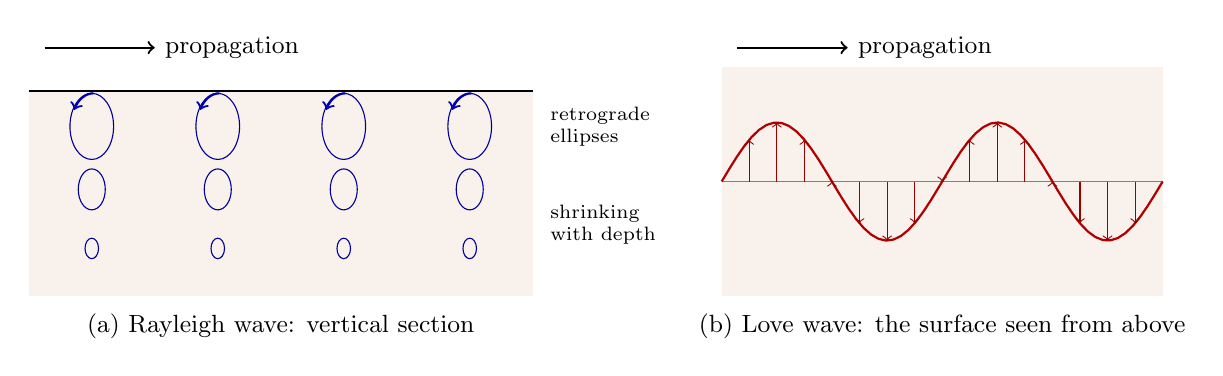
\begin{tikzpicture}[font=\small, x=1cm, y=1cm]
% Rayleigh: vertical section
\fill[brown!10] (0,0) rectangle (6.4,-2.6);
\draw[thick] (0,0) -- (6.4,0);
\draw[->, thick] (0.2,0.55) -- (1.6,0.55) node[right] {propagation};
\foreach \x/\s in {0.8/1, 2.4/-1, 4.0/1, 5.6/-1} {
  \foreach \z/\a in {-0.45/0.42, -1.25/0.26, -2.0/0.13} {
    \draw[blue!60!black] (\x,\z) ellipse ({0.66*\a} and {\a});
  }
}
\foreach \x in {0.8, 2.4, 4.0, 5.6} {
  \draw[->, blue!70!black, thick] (\x+0.02,-0.03) arc (90:150:{0.28} and {0.42});
}
\node[anchor=north] at (3.2,-2.7) {(a) Rayleigh wave: vertical section};
\node[anchor=west, font=\scriptsize, align=left] at (6.5,-0.45) {retrograde\\ellipses};
\node[anchor=west, font=\scriptsize, align=left] at (6.5,-1.7) {shrinking\\with depth};
% Love: plan view of the surface
\begin{scope}[xshift=8.8cm]
\fill[brown!10] (0,0.3) rectangle (5.6,-2.6);
\draw[->, thick] (0.2,0.55) -- (1.6,0.55) node[right] {propagation};
\draw[gray, thin] (0,-1.15) -- (5.6,-1.15);
\draw[red!70!black, thick, domain=0:5.6, samples=60] plot (\x,{-1.15+0.75*sin(\x*360/2.8)});
\foreach \x in {0.35,0.7,...,5.3} {
  \pgfmathsetmacro{\d}{0.75*sin(\x*360/2.8)}
  \draw[->, red!60!black] (\x,-1.15) -- (\x,{-1.15+\d});
}
\node[anchor=north] at (2.8,-2.7) {(b) Love wave: the surface seen from above};
\end{scope}
\end{tikzpicture}

\par\smallskip{\small Particle motions of the two surface waves (schematic).
(a) A \omterm{def:b3:seismology-imaging:surface-waves}{Rayleigh wave} moves the ground in the vertical plane of propagation,
along ellipses that turn backwards at the top (retrograde) near the surface and
shrink with depth. (b) A \omterm{def:b3:seismology-imaging:surface-waves}{Love wave} moves the ground horizontally, across the
direction of propagation: the arrows show the displacement at one instant
along a line of the surface.}
\label{fig:b3:seismology-imaging:particle-motion}
\end{omfigure}

\begin{theorem}[Dispersion of Love waves in a layer over a half-space]\label{thm:b3:seismology-imaging:love}
A layer of thickness $H$, shear modulus $\mu_1$ and S speed $\beta_1$ lies on a
half-space of shear modulus $\mu_2$ and S speed $\beta_2 > \beta_1$. A \omterm{def:b3:seismology-imaging:surface-waves}{Love
wave} of angular frequency $\omega$ and wave number $k$ propagates with the
phase velocity $c = \omega/k$, $\beta_1 < c < \beta_2$, if and only if
\[
  \tan\!\left(kH q_1\right) = \frac{\mu_2 q_2}{\mu_1 q_1},
  \qquad q_1 = \sqrt{\frac{c^2}{\beta_1^2} - 1},\quad
  q_2 = \sqrt{1 - \frac{c^2}{\beta_2^2}} .
\]
The fundamental mode is the root with $0 < kHq_1 < \pi/2$; the overtones have
$kHq_1$ in $(n\pi, n\pi + \pi/2)$.
\end{theorem}

\begin{proof}
Take $x$ along the propagation, $y$ horizontal across it and $z$ downwards from
the free surface, and look for a displacement
$u_y = f(z)\,e^{i(kx - \omega t)}$, the other components zero. Each layer
obeys the wave equation $\partial^2 u_y/\partial t^2 = \beta^2\nabla^2 u_y$, so
$f'' = -k^2\left(c^2/\beta^2 - 1\right) f$. In the layer, $c > \beta_1$, and
$f = A\cos(kq_1z) + B\sin(kq_1z)$. In the half-space, $c < \beta_2$, and the
solution that stays bounded at depth is $f = C\,e^{-kq_2(z - H)}$.
The shear traction on a horizontal plane is $\mu\,\partial u_y/\partial z$.
At the free surface it vanishes: $f'(0) = 0$, hence $B = 0$. At $z = H$ the
displacement and the traction are continuous:
\[
  A\cos(kq_1H) = C, \qquad -\mu_1 A\,kq_1\sin(kq_1H) = -\mu_2\,kq_2\,C .
\]
Dividing the second equation by the first gives the result. Since the
right-hand side is positive, $kHq_1$ lies in a quarter-period where the
tangent is positive; the smallest such interval gives the fundamental mode.
\end{proof}

For a given period the equation is solved for $c$ by bisection; the group
velocity follows from $U = \mathrm d\omega/\mathrm dk$. At short periods
($kH$ large) the root is near $c = \beta_1$: the wave lives in the layer. At
long periods ($kH \to 0$) it must have $kHq_1 \to 0$ with the right-hand side
small too, which forces $c \to \beta_2$: the wave reaches deep into the
half-space and travels at its speed. Between the two, the phase velocity rises
steadily with the period.

\begin{definition}[Surface-wave dispersion]\label{def:b3:seismology-imaging:dispersion}
\emph{Surface-wave dispersion}\index{surface-wave dispersion} is the dependence
of the phase and group velocities of a Rayleigh or \omterm{def:b3:seismology-imaging:surface-waves}{Love wave} on its period. In
a layered Earth it arises because a wave of longer period reaches deeper
(about a third of a wavelength for the fundamental mode) and averages faster
rock; the dispersion curves $c(T)$ and $U(T)$ measured between an earthquake
and a station, or between two stations, are inverted for the S speed as a
function of depth.
\end{definition}

\begin{omfigure}
\begin{tikzpicture}
\begin{axis}[omrecord, xmode=log, width=0.82\linewidth, height=0.5\linewidth,
  xmin=3, xmax=150, ymin=3.3, ymax=4.6, log basis x=10,
  xtick={3,5,10,20,50,100,150}, xticklabels={3,5,10,20,50,100,150},
  xlabel={period $T$ (\unit{s})}, ylabel={velocity (\unit{km.s^{-1}})},
  legend style={at={(0.03,0.62)}, anchor=west}, legend cell align=left]
\addplot[blue!70!black, thick] table[x=period, y=c] {figdata/out/bachelor-3-love_dispersion-curve.dat};
\addlegendentry{phase velocity $c$}
\addplot[red!70!black, thick] table[x=period, y=U] {figdata/out/bachelor-3-love_dispersion-curve.dat};
\addlegendentry{group velocity $U$}
\draw[gray, dashed] (axis cs:3,3.5) -- (axis cs:150,3.5);
\draw[gray, dashed] (axis cs:3,4.5) -- (axis cs:150,4.5);
\node[font=\scriptsize, anchor=south] at (axis cs:80,3.5) {$\beta_1 = 3.5$};
\node[font=\scriptsize, anchor=south west] at (axis cs:3.1,4.5) {$\beta_2 = 4.5$};
\addplot[only marks, mark=*, mark size=1.4pt, red!70!black] coordinates {(19.2,3.384)};
\node[font=\scriptsize, anchor=south, red!70!black] at (axis cs:19.2,3.39) {Airy phase};
\end{axis}
\end{tikzpicture}

\par\smallskip{\small Fundamental-mode \omterm{def:b3:seismology-imaging:surface-waves}{Love waves} in a \qty{35}{km} layer
($\beta_1 = \qty{3.5}{km.s^{-1}}$, \qty{2.7}{g.cm^{-3}}) on a half-space
($\beta_2 = \qty{4.5}{km.s^{-1}}$, \qty{3.3}{g.cm^{-3}}), a rounded model of a
continental crust on the mantle, computed from
\cref{thm:b3:seismology-imaging:love}. The phase velocity climbs from the
layer's S speed to the half-space's; the group velocity is lower and has a
minimum, \qty{3.384}{km.s^{-1}} at \qty{19.2}{s}, where waves of neighbouring
periods arrive together as a large late pulse (the Airy phase).}
\label{fig:b3:seismology-imaging:love}
\end{omfigure}

On this model the phase velocity at \qty{20}{s} is \qty{3.79}{km.s^{-1}} and at
\qty{100}{s} \qty{4.444}{km.s^{-1}}; the group velocities are 3.384 and
\qty{4.333}{km.s^{-1}}. On a seismogram recorded a few thousand kilometres
away, the long periods arrive first and the 20-s waves last, so that the
wave train is drawn out into a long, slowly shortening oscillation. Measuring
the group velocity at many periods along many paths gives maps of the crust's
thickness and of the uppermost mantle, independent of the body-wave travel
times.

\section{The Earth rings: normal modes}

A surface wave of very long period has a wavelength comparable to the Earth's
radius; it travels round the globe and meets itself. The waves that
interfere constructively are the standing waves of the whole sphere, its normal
modes, and after a great earthquake they are the last signal to die away.
Their theory, an eigenvalue problem for the elastic, self-gravitating Earth, is
beyond this chapter; their description is not.

The modes of a spherically symmetric Earth form two families. In the
\emph{toroidal} modes, ${}_nT_\ell$, the motion is horizontal, a twisting of
spherical shells against one another, with no change of radius or volume: the
standing waves of \omterm{def:b3:seismology-imaging:surface-waves}{Love waves}. In the \emph{spheroidal} modes, ${}_nS_\ell$,
the motion has radial and horizontal parts, and the Earth changes shape: the
standing waves of \omterm{def:b3:seismology-imaging:surface-waves}{Rayleigh waves}, coupled to the body waves and to gravity.
The index $\ell$ is the angular degree, the number of nodal lines of the
pattern on the surface; $n$ counts the nodes of the motion with radius, $n = 0$
for the fundamental mode. The gravest spheroidal mode, ${}_0S_2$, stretches the
Earth alternately into a prolate and an oblate spheroid; the gravest toroidal
mode, ${}_0T_2$, twists the northern and southern hemispheres in opposite
directions. Their observed periods are:
\begin{center}
\small
% ledger: seis5:modes-T, seis5:modes-S
\begin{tabular}{lcccc}
\hline
mode & ${}_0T_2$ & ${}_1T_2$ & ${}_0T_3$ & ${}_1T_3$ \\
period (\unit{min}) & 44.01 & 12.61 & 28.43 & 11.59 \\
\hline
mode & ${}_0S_2$ & ${}_1S_2$ & ${}_0S_3$ & ${}_1S_3$ \\
period (\unit{min}) & 53.89 & 24.51 & 35.56 & 17.68 \\
\hline
\end{tabular}
\end{center}
Each period is an average over the whole planet of its elastic moduli and
density, weighted by where the mode moves: the toroidal modes sense only the
solid mantle and crust, the spheroidal modes the core as well. Fitting the
periods of hundreds of modes is the only seismological way to weigh the
interior: it constrains the density, not only the speeds, and PREM was built to
fit them together with the travel times. The rotation and the ellipticity of
the Earth split each mode of degree $\ell$ into $2\ell + 1$ slightly different
frequencies, the analogue of the Zeeman effect.

\begin{history}[The Earth after the Chilean earthquake]
The 1960 Chilean earthquake was recorded by long-period pendulum seismometers
and by strainmeters, instruments that measure the change in length of a
long horizontal rod or wire anchored in rock. Spectral analysis of a few days of
record showed sharp peaks at the predicted periods of the gravest modes: the
whole Earth had been set ringing, and the predictions of the elastic theory
of a spherical, self-gravitating Earth were met. The record of the strainmeter
at Isabella, in California, was analysed again in 1978 with more modern
methods: it showed clearly the splitting of ${}_0T_3$, ${}_0T_4$, ${}_0S_4$
and ${}_0S_5$ by the rotation and ellipticity of the Earth, and confirmed that
of ${}_0S_2$ and ${}_0S_3$.
% ledger: stein78:chile-modes, usgs5:chile1960
Normal-mode seismology, born of one earthquake, now uses the networks of
very-broadband stations that record every great earthquake.
\end{history}

\section{Linear inverse problems}\label{sec:b3:seismology-imaging:inverse}

Every method of this chapter so far computes data from a model. The task of
imaging is the reverse.

\begin{definition}[Forward problem, inverse problem]\label{def:b3:seismology-imaging:inverse}
Let a model of the Earth be described by a vector $\mathbf m$ of $M$ parameters
and the observations by a vector $\mathbf d$ of $N$ data. The \emph{forward
problem}\index{forward problem} is to compute the data $\mathbf d = g(\mathbf m)$
that a given model would produce, by a physical theory. The \emph{inverse
problem}\index{inverse problem} is to estimate the model from data that carry
errors, $\mathbf d = g(\mathbf m) + \mathbf e$, and to say how well each part
of the model is determined. The problem is linear when $g(\mathbf m) =
\mathsf G\mathbf m$ for a fixed $N\times M$ matrix $\mathsf G$, the kernel.
\end{definition}

Fitting a straight line through travel times is a linear \omterm{def:b3:seismology-imaging:inverse}{inverse problem} with
$M = 2$ (exercise 7); a travel-time tomography is one with thousands of
parameters. Three cases arise. If $N > M$ and the data constrain every
parameter, the problem is \emph{overdetermined}: no model fits every datum
exactly, and the best is sought in a statistical sense. If some combination of
parameters leaves the data unchanged ($\mathsf G\mathbf m_0 = \mathbf 0$ for
some $\mathbf m_0 \ne \mathbf 0$), the problem is \emph{underdetermined} in that
direction, and no amount of data of that kind will fix it. Real problems are
mixed: overdetermined in some parts of the model and underdetermined in
others.

\begin{theorem}[Weighted least-squares estimate]\label{thm:b3:seismology-imaging:wls}
Let $\mathbf d = \mathsf G\mathbf m + \mathbf e$, where the errors $\mathbf e$
have zero mean and the covariance matrix $\mathsf C_d$ (diagonal
$\sigma_i^2$ for independent errors). If the matrix
$\mathsf N = \mathsf G^{\mathsf T}\mathsf C_d^{-1}\mathsf G$ is invertible, the
model that minimises the misfit
\[
  \chi^2(\mathbf m) = (\mathbf d - \mathsf G\mathbf m)^{\mathsf T}\mathsf C_d^{-1}
  (\mathbf d - \mathsf G\mathbf m)
\]
is the \emph{weighted least-squares estimate}\index{weighted least-squares estimate}
\[
  \hat{\mathbf m} = \mathsf N^{-1}\mathsf G^{\mathsf T}\mathsf C_d^{-1}\mathbf d ,
\]
it is unbiased, and its covariance matrix is
$\mathsf C_{\hat m} = \mathsf N^{-1}$.
\end{theorem}

\begin{proof}
$\chi^2$ is a quadratic function of $\mathbf m$ with gradient
$-2\mathsf G^{\mathsf T}\mathsf C_d^{-1}(\mathbf d - \mathsf G\mathbf m)$, which
vanishes for the normal equations $\mathsf N\mathbf m = \mathsf G^{\mathsf T}
\mathsf C_d^{-1}\mathbf d$; the Hessian $2\mathsf N$ is positive definite when
$\mathsf N$ is invertible (it is then $\mathbf x^{\mathsf T}\mathsf N\mathbf x =
\|\mathsf C_d^{-1/2}\mathsf G\mathbf x\|^2 > 0$ for $\mathbf x \ne 0$), so the
stationary point is the minimum. Write $\hat{\mathbf m} = \mathsf H\mathbf d$ with
$\mathsf H = \mathsf N^{-1}\mathsf G^{\mathsf T}\mathsf C_d^{-1}$. Then
$\mathsf H\mathsf G = \mathsf I$, so $\hat{\mathbf m} = \mathbf m + \mathsf H\mathbf e$
has mean $\mathbf m$, and its covariance is
$\mathsf H\mathsf C_d\mathsf H^{\mathsf T} =
\mathsf N^{-1}\mathsf G^{\mathsf T}\mathsf C_d^{-1}\mathsf C_d\mathsf C_d^{-1}
\mathsf G\mathsf N^{-1} = \mathsf N^{-1}$.
\end{proof}

The weights do what intuition asks: a datum with half the error counts four
times as much. The covariance matrix gives each parameter its standard error
$\sqrt{(\mathsf N^{-1})_{jj}}$ and the correlations between them. If the model
is right and the errors Gaussian, the minimum $\chi^2$ follows a $\chi^2$ law
with $N - M$ degrees of freedom: a value far above $N - M$ means the errors
were underestimated or the model is too simple; far below, that the errors
were overestimated.

When $\mathsf N$ is singular or nearly so, the estimate does not exist or is
dominated by noise amplified along the poorly constrained directions. The
standard remedy is to ask for a model that fits the data reasonably and is not
needlessly large.

\begin{definition}[Damped least squares, trade-off curve]\label{def:b3:seismology-imaging:damped}
For a damping parameter $\varepsilon > 0$, the \emph{damped least
squares}\index{damped least squares} estimate is the model that minimises
\[
  \Phi_\varepsilon(\mathbf m) = \chi^2(\mathbf m) + \varepsilon^2\|\mathbf m\|^2 ,
  \qquad
  \mathbf m_\varepsilon = \left(\mathsf N + \varepsilon^2\mathsf I\right)^{-1}
  \mathsf G^{\mathsf T}\mathsf C_d^{-1}\mathbf d .
\]
The \emph{trade-off curve}\index{trade-off curve} is the curve traced, as
$\varepsilon$ varies, by the pair (size of the model $\|\mathbf m_\varepsilon\|$,
misfit $\chi^2(\mathbf m_\varepsilon)$): small damping fits the data closely
with a large, rough model, large damping gives a small model and a poor fit.
\end{definition}

The formula is found as in \cref{thm:b3:seismology-imaging:wls}: the gradient
of $\Phi_\varepsilon$ is $-2\mathsf G^{\mathsf T}\mathsf C_d^{-1}(\mathbf d -
\mathsf G\mathbf m) + 2\varepsilon^2\mathbf m$, and $\mathsf N + \varepsilon^2
\mathsf I$ is always invertible, since its eigenvalues are those of
$\mathsf N$ (all $\ge 0$) increased by $\varepsilon^2$. The damping is usually
chosen near the knee of the \omterm{def:b3:seismology-imaging:damped}{trade-off curve}, or so that $\chi^2$ is about the
number of data, the misfit expected from the errors alone. The price is that the
estimate is no longer unbiased.

\begin{definition}[Model resolution matrix]\label{def:b3:seismology-imaging:resolution}
For a linear estimate $\mathbf m_\varepsilon = \mathsf H_\varepsilon \mathbf d$
of the model $\mathbf m$ from data $\mathbf d = \mathsf G\mathbf m + \mathbf e$,
the \emph{model resolution matrix}\index{model resolution matrix} is
$\mathsf R = \mathsf H_\varepsilon\mathsf G$, so that
\[
  \mathbf m_\varepsilon = \mathsf R\,\mathbf m + \mathsf H_\varepsilon\mathbf e .
\]
For \omterm{def:b3:seismology-imaging:damped}{damped least squares}, $\mathsf R = (\mathsf N + \varepsilon^2\mathsf I)^{-1}
\mathsf N$. Row $j$ of $\mathsf R$ shows how the estimate of parameter $j$
averages the true parameters; $\mathsf R = \mathsf I$ means perfect resolution.
\end{definition}

If $\mathsf N$ has the orthonormal eigenvectors $\mathbf u_k$ and eigenvalues
$\lambda_k$, then $\mathsf R = \sum_k \frac{\lambda_k}{\lambda_k + \varepsilon^2}
\mathbf u_k\mathbf u_k^{\mathsf T}$: the directions the data constrain well
($\lambda_k \gg \varepsilon^2$) pass almost unchanged, those they constrain
poorly are suppressed. The trace of $\mathsf R$ counts the parameters the data
effectively resolve, and the covariance of the estimate,
$\mathsf H_\varepsilon\mathsf C_d\mathsf H_\varepsilon^{\mathsf T}$, shrinks as
the resolution does: damping trades resolution for stability.

\begin{omfigure}
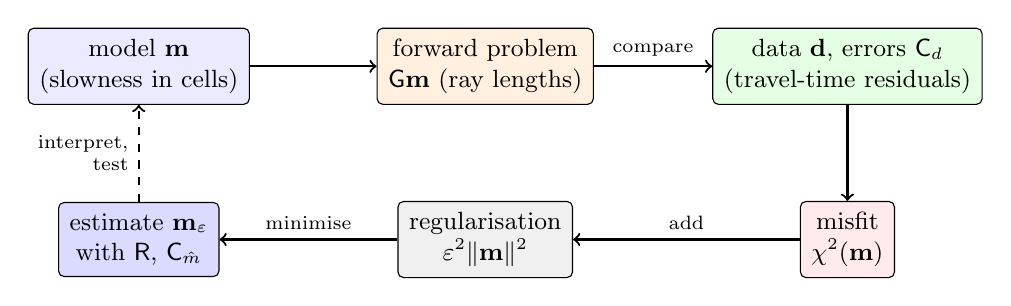
\begin{tikzpicture}[font=\small, node distance=0.5cm,
  box/.style={draw, rounded corners=2pt, fill=#1, minimum height=0.9cm, align=center, inner sep=4pt},
  box/.default=gray!8]
\node[box=blue!8] (m) at (0,0) {model $\mathbf m$\\(slowness in cells)};
\node[box=orange!12] (g) at (4.4,0) {forward problem\\$\mathsf G\mathbf m$ (ray lengths)};
\node[box=green!10] (d) at (9.0,0) {data $\mathbf d$, errors $\mathsf C_d$\\(travel-time residuals)};
\node[box=red!8] (mis) at (9.0,-2.2) {misfit\\$\chi^2(\mathbf m)$};
\node[box=gray!12] (reg) at (4.4,-2.2) {regularisation\\$\varepsilon^2\|\mathbf m\|^2$};
\node[box=blue!14] (est) at (0,-2.2) {estimate $\mathbf m_\varepsilon$\\with $\mathsf R$, $\mathsf C_{\hat m}$};
\draw[->, thick] (m) -- (g);
\draw[->, thick] (g) -- node[above, font=\scriptsize] {compare} (d);
\draw[->, thick] (d) -- (mis);
\draw[->, thick] (mis) -- node[above, font=\scriptsize] {add} (reg);
\draw[->, thick] (reg) -- node[above, font=\scriptsize] {minimise} (est);
\draw[->, thick, dashed] (est) -- node[left, font=\scriptsize, align=right] {interpret,\\test} (m);
\end{tikzpicture}

\par\smallskip{\small The linear \omterm{def:b3:seismology-imaging:inverse}{inverse problem} as a loop (schematic). The
\omterm{def:b3:seismology-imaging:inverse}{forward problem} predicts data from a model; the misfit, weighted by the data
errors, measures the disagreement; the regularisation term keeps the model
small; minimising their sum gives the estimate, which is only interpretable
together with its resolution matrix and covariance.}
\label{fig:b3:seismology-imaging:inverse-loop}
\end{omfigure}

\section{Seismic tomography}\label{sec:b3:seismology-imaging:tomography}

\begin{definition}[Seismic tomography, travel-time residual]\label{def:b3:seismology-imaging:tomography}
The \emph{travel-time residual}\index{travel-time residual} of an arrival is the
observed travel time minus the time predicted by a reference model,
$\delta t = T_{\text{obs}} - T_{\text{ref}}$, after correction for the source
location and origin time, the station's elevation and the Earth's
ellipticity. \emph{Seismic tomography}\index{seismic tomography} is the
estimation of the three-dimensional departures of the seismic speeds from a
reference model, $\delta v(\mathbf x)$, from a large set of residuals (or of
waveforms), by solving an \omterm{def:b3:seismology-imaging:inverse}{inverse problem}.
\end{definition}

Write $s = 1/v$ for the slowness. The travel time along a ray $\Gamma$ is
$T = \int_\Gamma s\,\mathrm dl$; but the ray itself depends on the speeds,
which seems to make the problem non-linear. The first-order answer is that it
does not matter.

\begin{proposition}[Linearised travel-time residual]\label{prop:b3:seismology-imaging:linear}
If the slowness of the reference model $s_0$ is perturbed to $s_0 + \delta s$,
the travel time between two fixed points changes, to first order in
$\delta s$, by
\[
  \delta t = \int_{\Gamma_0}\delta s\,\mathrm dl ,
\]
the integral being taken along the ray $\Gamma_0$ of the reference model; the
relative speed anomaly is $\delta v/v_0 = -\delta s/s_0$ to the same order.
\end{proposition}

\begin{proof}
By Fermat's principle the ray $\Gamma_0$ makes the travel time
$\int s_0\,\mathrm dl$ stationary among neighbouring paths: moving the path by a
small amount $\epsilon$ changes the time by a term of order $\epsilon^2$ only.
The new ray $\Gamma$ differs from $\Gamma_0$ by an amount of order $\delta s$;
so $\int_\Gamma(s_0 + \delta s)\,\mathrm dl = \int_{\Gamma_0}s_0\,\mathrm dl +
O(\delta s^2) + \int_{\Gamma_0}\delta s\,\mathrm dl + O(\delta s^2)$. Finally
$\delta(1/s) = -\delta s/s_0^2$, so $\delta v/v_0 = -\delta s/s_0$.
\end{proof}

Cut the region into $M$ cells of uniform slowness perturbation $\delta s_j$.
The residual of ray $i$ becomes $\delta t_i = \sum_j L_{ij}\,\delta s_j$, where
$L_{ij}$ is the length of the reference ray $i$ in cell $j$: a linear \omterm{def:b3:seismology-imaging:inverse}{inverse
problem} whose kernel is the matrix of ray lengths, almost all of whose entries
are zero. The residuals are small: in a mantle at
\qty{8}{km.s^{-1}}, a region \qty{200}{km} across that is \qty{3}{\percent}
faster advances a vertical ray by about \qty{0.7}{s} (exercise 9).

\begin{method}[A travel-time tomography]\label{met:b3:seismology-imaging:tomo}
\begin{enumerate}
  \item Pick the arrival times of one phase (say P) at all stations, for
        earthquakes whose location is well known; compute the residuals
        against a \omterm{def:b3:seismology-imaging:tables}{travel-time table}, corrected for ellipticity and station
        elevation.
  \item Trace the reference rays and cut the region into cells (or expand
        $\delta s$ on smooth functions); fill the matrix of ray lengths.
  \item Assign each residual its error, from the picking precision, and solve
        the damped least-squares problem for a range of damping values; draw
        the \omterm{def:b3:seismology-imaging:damped}{trade-off curve} and choose the damping near its knee.
  \item Test the resolution: compute the residuals that a known synthetic
        model would give through the same rays, add noise, invert them with the
        same damping, and compare.
  \item Interpret only the anomalies that the test shows the rays can
        recover, with their amplitudes understood as lower bounds.
\end{enumerate}
\end{method}

\begin{definition}[Checkerboard test]\label{def:b3:seismology-imaging:checkerboard}
A \emph{checkerboard test}\index{checkerboard test} is a resolution test in
which the synthetic model is a regular pattern of alternately fast and slow
cells: synthetic residuals computed through the real ray geometry, with noise
of the size of the real errors, are inverted with the same parametrisation and
damping. Where the pattern is recovered, structures of that size can be
resolved; where it is smeared or lost, they cannot.
\end{definition}

The figures below run the test on a model section \qty{800}{km} wide and
\qty{400}{km} deep, cut into 128 cells of \qty{50}{km}. Twenty sources lie
along its base and thirty-two stations along its top, and only the rays within
\ang{45} of the vertical are used: 480 rays that all travel steeply upwards,
the geometry of rays from distant earthquakes rising beneath a network. The
synthetic model has blocks of $2\times2$ cells, \qty{3}{\percent} fast or slow
around \qty{8}{km.s^{-1}}; the residuals carry Gaussian noise of
\qty{0.05}{s}.
% figdata: tomo_checkerboard.py (invented geometry; no real data)

\begin{omfigure}
\begin{tikzpicture}
\begin{groupplot}[group style={group size=2 by 2, horizontal sep=0.9cm, vertical sep=1.25cm},
  width=0.46\linewidth, height=0.3\linewidth, xmin=0, xmax=800, ymin=0, ymax=400,
  axis on top, enlargelimits=false, tick label style={font=\scriptsize},
  title style={font=\small, yshift=-1ex},
  colormap={tomo}{rgb255(0cm)=(178,24,43); rgb255(1cm)=(244,165,130); rgb255(2cm)=(247,247,247); rgb255(3cm)=(146,197,222); rgb255(4cm)=(33,102,172)},
  point meta min=-4, point meta max=4]
\nextgroupplot[title={(a) synthetic model}, ylabel={\scriptsize height (km)}]
\addplot[matrix plot*, mesh/cols=16, point meta=explicit] table[x=x, y=y, meta=dv] {figdata/out/bachelor-3-tomo_checkerboard-true.dat};
\nextgroupplot[title={(b) a sample of the 480 rays}, colormap/blackwhite]
\addplot[gray!70!black, thin, unbounded coords=jump] table[x=x, y=y] {figdata/out/bachelor-3-tomo_checkerboard-rays.dat};
\addplot[only marks, mark=triangle*, mark size=1.6pt, black, clip=false] table[x=x, y=y] {figdata/out/bachelor-3-tomo_checkerboard-receivers.dat};
\addplot[only marks, mark=star, mark size=1.8pt, red!70!black, clip=false] table[x=x, y=y] {figdata/out/bachelor-3-tomo_checkerboard-sources.dat};
\nextgroupplot[title={(c) recovered, $\varepsilon = \qty{3}{km}$}, ylabel={\scriptsize height (km)}, xlabel={\scriptsize distance (km)}]
\addplot[matrix plot*, mesh/cols=16, point meta=explicit] table[x=x, y=y, meta=dv] {figdata/out/bachelor-3-tomo_checkerboard-rec-low.dat};
\nextgroupplot[title={(d) recovered, $\varepsilon = \qty{60}{km}$}, xlabel={\scriptsize distance (km)},
  colorbar right, colorbar style={width=0.2cm, ytick={-4,-2,0,2,4}, ylabel={\scriptsize $\delta v/v$ (\%)}, tick label style={font=\scriptsize}}]
\addplot[matrix plot*, mesh/cols=16, point meta=explicit] table[x=x, y=y, meta=dv] {figdata/out/bachelor-3-tomo_checkerboard-rec-high.dat};
\end{groupplot}
\end{tikzpicture}

\par\smallskip{\small A \omterm{def:b3:seismology-imaging:checkerboard}{checkerboard test} (invented geometry). (a) The
synthetic model: blocks \qty{100}{km} across, \qty{3}{\percent} fast (blue) or
slow (red). (b) The 20 sources (stars), the 32
stations (triangles) and some of the rays, all within \ang{45} of the vertical. (c) With
light damping the blocks are found, but noisy, with anomalies up to about
\qty{8}{\percent} where few rays cross (colours saturate at
\qty{4}{\percent}). (d) With heavy damping the pattern is clean, but its
amplitude is reduced, most of all along the side edges, where few rays cross
and all at similar angles.}
\label{fig:b3:seismology-imaging:checkerboard}
\end{omfigure}

\begin{omfigure}
\begin{tikzpicture}
\begin{axis}[omrecord, width=0.62\linewidth, height=0.42\linewidth,
  xlabel={model norm $\|\delta v/v\|$ (\unit{\percent})},
  ylabel={misfit $\|\mathsf G\mathbf m - \mathbf d\|$ (\unit{s})}, xmin=0, xmax=42, ymin=0, ymax=12]
\addplot[blue!70!black, thick] table[x=norm, y=misfit] {figdata/out/bachelor-3-tomo_checkerboard-tradeoff.dat};
\addplot[only marks, mark=*, mark size=1.8pt, red!70!black] coordinates {(38.84,0.862) (29.42,1.159)};
\node[font=\scriptsize, anchor=south, red!70!black] at (axis cs:38.84,1.3) {$\varepsilon = 3$};
\node[font=\scriptsize, anchor=east, red!70!black] at (axis cs:28.6,0.55) {$\varepsilon = 60$};
\draw[gray, dashed] (axis cs:0,1.095) -- (axis cs:42,1.095);
\node[font=\scriptsize, anchor=south west] at (axis cs:1,1.15) {expected from the noise};
\draw[green!45!black, densely dotted] (axis cs:33.94,0) -- (axis cs:33.94,12);
\node[font=\scriptsize, anchor=north west, green!45!black] at (axis cs:34.2,11.8) {true model};
\node[font=\scriptsize, anchor=west] at (axis cs:14,10.5) {heavy damping};
\node[font=\scriptsize, anchor=east] at (axis cs:41,3.2) {light damping};
\end{axis}
\end{tikzpicture}

\par\smallskip{\small The \omterm{def:b3:seismology-imaging:damped}{trade-off curve} of the \omterm{def:b3:seismology-imaging:checkerboard}{checkerboard test}, for damping
values $\varepsilon$ from 0.1 to \qty{1000}{km} (the kernel is in kilometres,
with equal errors). Along the flat part, more damping costs almost no fit: the
model shrinks by losing noise. The knee lies where the misfit rises through the
level expected from the noise alone, $\sigma\sqrt{480} = \qty{1.095}{s}$; the
two damped models of the previous figure lie on either side of it, and the
norm of the true checkerboard, \qty{33.9}{\percent}, between them. Beyond the
knee the damping removes structure the data require.}
\label{fig:b3:seismology-imaging:tradeoff}
\end{omfigure}

The test illustrates the three limits of every tomographic image. Resolution
is set by the rays: where all rays are parallel, an anomaly is smeared along
them, and a cell crossed by few rays is barely constrained. Damping lowers the
amplitudes: the recovered anomalies are lower bounds.
And the image depends on the reference model and the parametrisation: only the
departures from the reference are mapped, and nothing smaller than a cell.
With these cautions, the global P- and S-wave images show the slabs of the
Year 1 volume (in its chapter on subduction) as tabular fast regions descending
from the trenches, some flattening above the 670-km discontinuity, others
plunging into the lower mantle; and broad slow regions under the Pacific and
Africa above the core, with narrower slow conduits beneath some hotspots, the
candidates for the mantle plumes of the same volume.

\begin{inthefield}[A broadband station and an ocean-bottom deployment]
\begin{minipage}[t]{0.55\linewidth}\vspace{0pt}
A permanent broadband station is a quiet place: the seismometer stands on a
concrete pier bolted to bedrock in a buried vault or a short tunnel, under a
thermal shield, because a draught or a change of a few hundredths of a degree
tilts the instrument more than a distant earthquake. Its three components,
vertical, north and east, are digitised continuously and sent to a data centre
with a satellite time stamp. To image a region beneath the ocean, a survey team
instead drops ocean-bottom seismometers from a ship: each sinks on an anchor,
records for a year on the sea floor, and returns to the surface when the ship
comes back and sends an acoustic signal to release it. The crew then reads its
clock drift, corrects the records, and adds thousands of arrivals to the
tomography.
\end{minipage}\hfill
\begin{minipage}[t]{0.42\linewidth}\vspace{0pt}
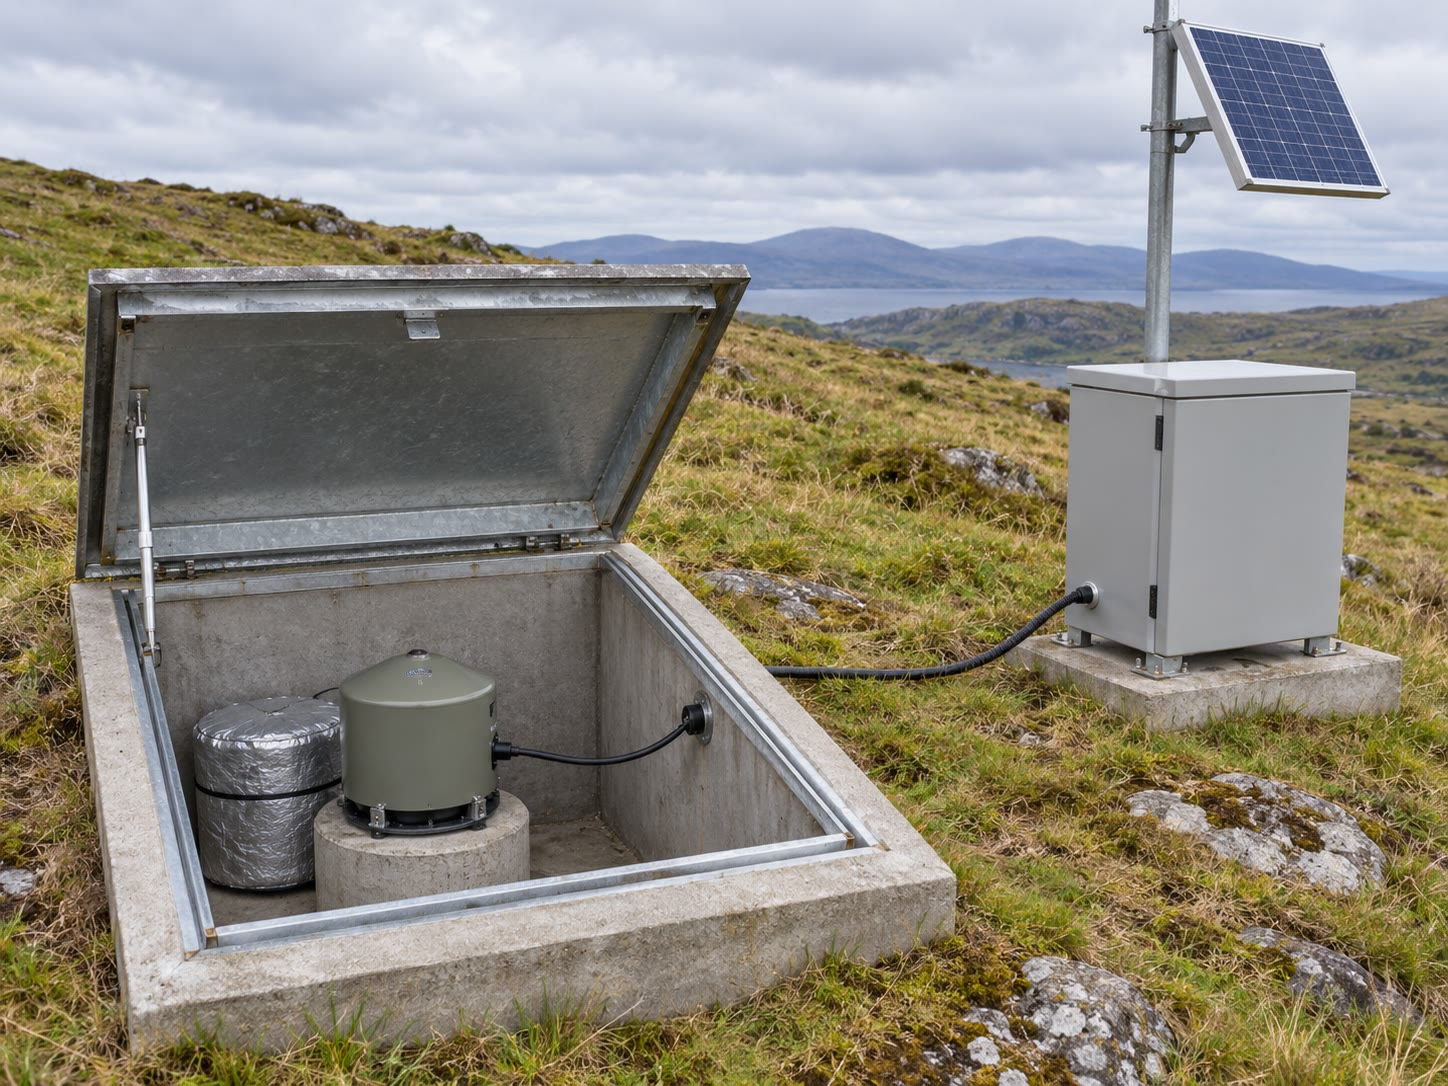
\includegraphics[width=\linewidth]{images/book5/ai/b3-seismic-vault.jpg}

{\scriptsize A broadband seismometer on its pier in a station vault
(AI-generated illustration).}
\end{minipage}
\end{inthefield}

\section{Exercises}

\begin{exercise}[$\star$]\label{exo:b3:seismology-imaging:1}
A P ray leaves the surface ($R = \qty{6371}{km}$, $v_0 = \qty{5.80}{km.s^{-1}}$)
with the \omterm{def:b3:seismology-imaging:ray-parameter}{ray parameter} $p = \qty{500}{s.rad^{-1}}$. (a) Compute its take-off
angle. (b) PREM gives P speeds of \qty{11.066}{km.s^{-1}} at \qty{771}{km} depth
and \qty{11.245}{km.s^{-1}} at \qty{871}{km}. Compute $r/v$ at both depths and
find the turning depth of the ray by linear interpolation.
% ledger: ak135:crust, data:prem
\end{exercise}

\begin{exercise}[$\star$]\label{exo:b3:seismology-imaging:2}
The P times computed through PREM in this chapter are \qty{369.6}{s} at \ang{30}
and \qty{455.5}{s} at \ang{40}. (a) Estimate the slope of the travel-time
curve between them, in \unit{s} per degree and in \unit{s.rad^{-1}}. (b) Deduce
the apparent speed of the wave front along the surface, in
\unit{km.s^{-1}}. (c) What is the P speed at the turning point of the ray
arriving at \ang{35}, if it turns at the radius \qty{5450}{km}?
\end{exercise}

\begin{exercise}[$\star$]\label{exo:b3:seismology-imaging:3}
In the Love-wave model of this chapter the layer has $\beta_1 =
\qty{3.5}{km.s^{-1}}$, $\rho_1 = \qty{2700}{kg.m^{-3}}$ and the half-space
$\beta_2 = \qty{4.5}{km.s^{-1}}$, $\rho_2 = \qty{3300}{kg.m^{-3}}$.
(a) Compute the two shear moduli. (b) At \qty{20}{s} the phase velocity is
\qty{3.79}{km.s^{-1}}: compute the wavelength and compare it with the layer
thickness, \qty{35}{km}. (c) With group velocities of \qty{3.384}{km.s^{-1}} at
\qty{20}{s} and \qty{4.333}{km.s^{-1}} at \qty{100}{s}, by how many minutes do
the 20-s waves arrive after the 100-s waves at a station \qty{4000}{km} away?
\end{exercise}

\begin{exercise}[$\star$]\label{exo:b3:seismology-imaging:4}
The observed periods of ${}_0S_2$ and ${}_0T_2$ are \qty{53.89}{min} and
\qty{44.01}{min}. (a) Compute their frequencies in \unit{mHz}. (b) How many
oscillations of each does the Earth complete in a day? (c) Two spectral peaks
can be separated only if the record lasts at least the inverse of their
frequency difference. How long must a record be to separate these two modes?
% ledger: seis5:modes-S, seis5:modes-T
\end{exercise}

\begin{exercise}[$\star\star$]\label{exo:b3:seismology-imaging:5}
In a sphere of radius $R$ and uniform speed $v$ the rays are straight chords.
(a) Show that the ray reaching $\Delta$ has the travel time
$T = 2R\sin(\Delta/2)/v$. (b) With $R = \qty{6371}{km}$ and
$v = \qty{10.0}{km.s^{-1}}$, compute $T$ at \ang{30} and \ang{90}, and compare
with the PREM times, \qty{369.6}{s} and \qty{779.7}{s}. (c) Explain why the
uniform sphere is too fast at \ang{30} and too slow at \ang{90}.
\end{exercise}

\begin{exercise}[$\star\star$]\label{exo:b3:seismology-imaging:6}
On a Poisson solid ($\lambda = \mu$, so $\alpha^2 = 3\beta^2$) the \omterm{def:b3:seismology-imaging:surface-waves}{Rayleigh wave}
speed $c$ satisfies, with $\xi = c^2/\beta^2$,
$(2 - \xi)^2 = 4\sqrt{1 - \xi/3}\,\sqrt{1 - \xi}$. (a) Square it and show
that the roots satisfy $(\xi - 4)(3\xi^2 - 12\xi + 8) = 0$. (b) Show that the
only root with $0 < \xi < 1$ is $\xi = 2 - 2/\sqrt3$, and compute $c/\beta$.
(c) In the ak135 upper crust, $\beta = \qty{3.46}{km.s^{-1}}$: compute the
Rayleigh speed and the delay of the \omterm{def:b3:seismology-imaging:surface-waves}{Rayleigh wave} behind the S wave at
\qty{1000}{km}.
% ledger: ak135:crust
\end{exercise}

\begin{exercise}[$\star\star$]\label{exo:b3:seismology-imaging:7}
Head-wave arrivals at four stations of a refraction line, at 50, 100, 150 and
\qty{200}{km} from the shot, are 9.0, 15.3, 21.5 and \qty{27.9}{s}, with
errors of 0.1, 0.1, 0.2 and \qty{0.2}{s}. Fit $T = a + bx$ by weighted least
squares: write $\mathsf G$ and $\mathsf C_d$, form the normal equations, and
give $a$, $b$, their standard errors, the speed $1/b$ with its error, and the
minimum $\chi^2$. Is the fit acceptable?
\end{exercise}

\begin{exercise}[$\star\star$]\label{exo:b3:seismology-imaging:8}
One ray crosses two cells, with lengths \qty{30}{km} and \qty{40}{km}, and has
a residual of \qty{0.50}{s}. (a) Why is $\mathsf N = \mathsf G^{\mathsf T}
\mathsf G$ singular? (b) Among the models that fit the residual exactly, the one
of smallest norm is $\mathbf m = \mathsf G^{\mathsf T}(\mathsf G\mathsf
G^{\mathsf T})^{-1}\mathbf d$: compute it. (c) Compute the matrix
$\mathsf R = \mathsf G^{\mathsf T}(\mathsf G\mathsf G^{\mathsf T})^{-1}\mathsf G$
and its trace. (d) If the true anomaly is \qty{0.01}{s.km^{-1}} in the first
cell only, what is recovered?
\end{exercise}

\begin{exercise}[$\star\star$]\label{exo:b3:seismology-imaging:9}
A slab region of the mantle is \qty{3}{\percent} faster than its surroundings,
where $v = \qty{9.0}{km.s^{-1}}$. (a) Compute the residual of a ray crossing
\qty{200}{km} of it vertically, by \cref{prop:b3:seismology-imaging:linear},
and exactly. (b) The same for a ray crossing a \qty{100}{km} thickness of it at
\ang{40} from the normal to the slab. (c) What is the relative error of the
linearisation?
\end{exercise}

\begin{exercise}[$\star\star\star$]\label{exo:b3:seismology-imaging:10}
In \cref{thm:b3:seismology-imaging:love}, an overtone of order $n$ exists only
at periods short enough. (a) Show that at its cut-off its phase velocity is
$\beta_2$ and $kHq_1 = n\pi$. (b) Deduce the cut-off angular frequency
$\omega_n = n\pi\beta_1\beta_2/\bigl(H\sqrt{\beta_2^2 - \beta_1^2}\bigr)$.
(c) Compute the cut-off period of the first overtone for the chapter's model
($H = \qty{35}{km}$, $\beta_1 = 3.5$, $\beta_2 = \qty{4.5}{km.s^{-1}}$).
(d) Show that the fundamental mode has no cut-off, and that its phase velocity
tends to $\beta_1$ at short periods.
\end{exercise}

\begin{exercise}[$\star\star\star$]\label{exo:b3:seismology-imaging:11}
Take the ray of exercise 8, with unit data error. (a) Show that, for any
$\varepsilon > 0$, $(\mathsf G^{\mathsf T}\mathsf G + \varepsilon^2\mathsf
I)^{-1}\mathsf G^{\mathsf T} = \mathsf G^{\mathsf T}(\mathsf G\mathsf
G^{\mathsf T} + \varepsilon^2\mathsf I)^{-1}$. (b) Deduce the damped resolution
matrix $\mathsf R_\varepsilon = \mathsf G^{\mathsf T}\mathsf G/(\|\mathbf g\|^2 +
\varepsilon^2)$, where $\mathbf g = (30, 40)$, and its trace. (c) Compute the
trace and the data residual for $\varepsilon^2 = 0$, 2500 and \num{10000}
(in \unit{km^2}). Describe the trade-off.
\end{exercise}

\begin{exercise}[$\star\star\star$]\label{exo:b3:seismology-imaging:12}
In the uniform sphere of exercise 5: (a) show by
\cref{thm:b3:seismology-imaging:benndorf} that $p(\Delta) = (R/v)\cos(\Delta/2)$,
and check it against the definition of $p$ (the take-off angle of a chord).
(b) Show that the ray reaching $\Delta_1$ turns at $r_1 = R\cos(\Delta_1/2)$.
(c) Admitting that $\int_0^{\Delta_1}\operatorname{arccosh}\bigl(\cos(\Delta/2)
/\cos(\Delta_1/2)\bigr)\,\mathrm d\Delta = \pi\ln\bigl(1/\cos(\Delta_1/2)\bigr)$,
show that the Herglotz--Wiechert formula returns $r_1$ and the speed $v$.
\end{exercise}

\section{Problem: The Slab beneath Station K}

\begin{problem}[{Weekend problem --- rays, Love waves and a small tomography
beneath an invented station}]
\label{pb:b3:seismology-imaging:1}
% values: calc/ch01.py (invented station and models; Love-wave model as in the chapter)
Station K stands on a continent above a subduction zone. This problem uses its
records three ways: rays in its crust, the dispersion of \omterm{def:b3:seismology-imaging:surface-waves}{Love waves} across it,
and a small tomography of the mantle below.

\medskip
\noindent\textbf{Part I --- Rays in a gradient.} Over distances short enough to
neglect the Earth's curvature, the P speed beneath K rises linearly with depth,
$v(z) = v_0 + gz$, with $v_0 = \qty{5.0}{km.s^{-1}}$ and
$g = \qty{0.05}{s^{-1}}$ ($z$ in km).
\begin{enumerate}
  \item In flat layers, Snell's law keeps $p = \sin i/v$ constant. A ray leaves
        K with $\sin i_0 = 0.8$: compute $i_0$ and $p$.
  \item At what depth does it turn, and what is the speed there?
  \item Show that $\mathrm di/\mathrm ds = pg$ along the ray, so that it is an
        arc of circle; give its radius and the depth of its centre.
  \item Compute the horizontal distance $X$ at which the ray returns to the
        surface.
  \item Show that $\mathrm dT = \mathrm di/(g\sin i)$ and compute the travel
        time $T$ exactly.
  \item Compute $X$ and $T$ for $p = \qty{0.15}{s.km^{-1}}$, and check that
        $\Delta T/\Delta X$ between the two rays lies between the two values
        of $p$.
\end{enumerate}

\noindent\textbf{Part II --- Love waves and the crust.} The crust under K is a
layer of S speed $\beta_1 = \qty{3.5}{km.s^{-1}}$ and density
$\rho_1 = \qty{2.7}{g.cm^{-3}}$ over a mantle with $\beta_2 =
\qty{4.5}{km.s^{-1}}$, $\rho_2 = \qty{3.3}{g.cm^{-3}}$; its thickness $H$ is
unknown. Between K and a neighbouring station the Love-wave phase velocity is
measured: \qty{3.99}{km.s^{-1}} at \qty{25}{s} and \qty{4.25}{km.s^{-1}} at
\qty{40}{s}.
\begin{enumerate}[resume]
  \item Compute $\mu_1$ and $\mu_2$ in \unit{GPa}.
  \item At \qty{25}{s}, compute $k$, $q_1$ and $q_2$.
  \item Solve the dispersion equation of the fundamental mode for $H$.
  \item Do the same at \qty{40}{s}. Are the two results consistent?
  \item Estimate the group velocity between the two periods as
        $\Delta\omega/\Delta k$, and compare it with the phase velocities.
  \item Compute the wavelength at each period, and explain why the two
        periods sense the crust and the uppermost mantle in different
        proportions.
\end{enumerate}

\noindent\textbf{Part III --- A tomography in four cells.} Below K, a block of
mantle \qty{200}{km} by \qty{200}{km} in a vertical section is cut into four
square cells of \qty{100}{km}: 1 (upper left), 2 (upper right), 3 (lower left)
and 4 (lower right); the trench and the ocean lie to the left. The reference speed is $v_0 = \qty{8.0}{km.s^{-1}}$. In an
idealised experiment six straight rays cross it: A along the upper row (cells 1
and 2), B along the lower row (3 and 4), C down the left column (1 and 3), D
down the right column (2 and 4), E along the diagonal through 1 and 4, F along
the diagonal through 2 and 3. Their residuals are:
\begin{center}
\small
\begin{tabular}{lcccccc}
\hline
ray & A & B & C & D & E & F \\
$\delta t$ (\unit{s}) & $0.16$ & $-0.48$ & $-0.36$ & $0.11$ & $-0.15$ & $-0.27$ \\
error $\sigma$ (\unit{s}) & 0.05 & 0.05 & 0.05 & 0.05 & 0.10 & 0.10 \\
\hline
\end{tabular}
\end{center}
Take the model $\mathbf m$ as the slowness perturbations of the cells in
\unit{ms.km^{-1}} ($\qty{1}{ms.km^{-1}} = \qty{e-3}{s.km^{-1}}$), so that the
entries of $\mathsf G$ are the ray lengths in \unit{km} divided by 1000.
\begin{enumerate}[resume]
  \item Write $\mathsf G$, a $6\times4$ matrix.
  \item Show that $\mathsf N = \mathsf G^{\mathsf T}\mathsf C_d^{-1}\mathsf G$
        has the rows $(10, 4, 4, 2)$, $(4, 10, 2, 4)$, $(4, 2, 10, 4)$,
        $(2, 4, 4, 10)$.
  \item Compute $\mathbf b = \mathsf G^{\mathsf T}\mathsf C_d^{-1}\mathbf d$.
  \item Check that $(1,1,1,1)$, $(1,-1,-1,1)$, $(1,1,-1,-1)$ and $(1,-1,1,-1)$
        are eigenvectors of $\mathsf N$, with eigenvalues 20, 4, 8 and 8, and
        deduce that $\mathsf N^{-1}$ has the rows $(11, -4, -4, 1)/80$,
        $(-4, 11, 1, -4)/80$, $(-4, 1, 11, -4)/80$ and $(1, -4, -4, 11)/80$.
  \item Compute the \omterm{thm:b3:seismology-imaging:wls}{weighted least-squares estimate} $\hat{\mathbf m}$.
  \item Convert it into relative speed anomalies $\delta v/v_0$ in per cent.
  \item Give the standard error of each cell in \unit{ms.km^{-1}} and in per
        cent, and the correlation between cells 1 and 2, and between cells 1
        and 4. Explain their signs.
  \item Compute the residuals of the six rays after the fit and the minimum
        $\chi^2$. Is it consistent with the stated errors?
\end{enumerate}

\noindent\textbf{Part IV --- Damping, resolution and the slab.}
\begin{enumerate}[resume]
  \item For $\varepsilon^2 = 4$ (in the units of $\mathsf N$), give the
        eigenvalues of $\mathsf R = (\mathsf N + 4\mathsf I)^{-1}\mathsf N$ and
        show that $\mathsf R$ has the diagonal $2/3$, the entries $1/12$
        between cells that share a row or column ray, and $0$ between cells 1
        and 4 and between cells 2 and 3.
  \item Compute the damped estimate of cell 3 and its speed anomaly. Why is it
        smaller than the undamped one?
  \item The damped model has $\chi^2 = 15.8$ and norm \qty{2.91}{ms.km^{-1}};
        the undamped, $\chi^2 = 0.50$ and \qty{4.24}{ms.km^{-1}}. Which would
        you keep, and why does this problem not need damping?
  \item Read row 3 of the damped $\mathsf R$: with which cells is the estimate
        of cell 3 blurred?
  \item Which cell is fast, and which slow? Interpret the fast cell, below and
        on the ocean side of K, in terms of the subduction zone.
  \item Give the P-velocity anomaly of the slab cell in per cent, with its
        standard error.
\end{enumerate}
\end{problem}
